\chapter{Конструкторский раздел}
\label{cha:design}

В данном разделе будет проведена конкретизация поставленных задач, составлены и проанализированы алгоритмы.

\section{Функциональная модель}
На рисунке \ref{img:IDEF0} представлена функциональная модель IDEF0 уровня 1.
\begin{figure}
    \centering
    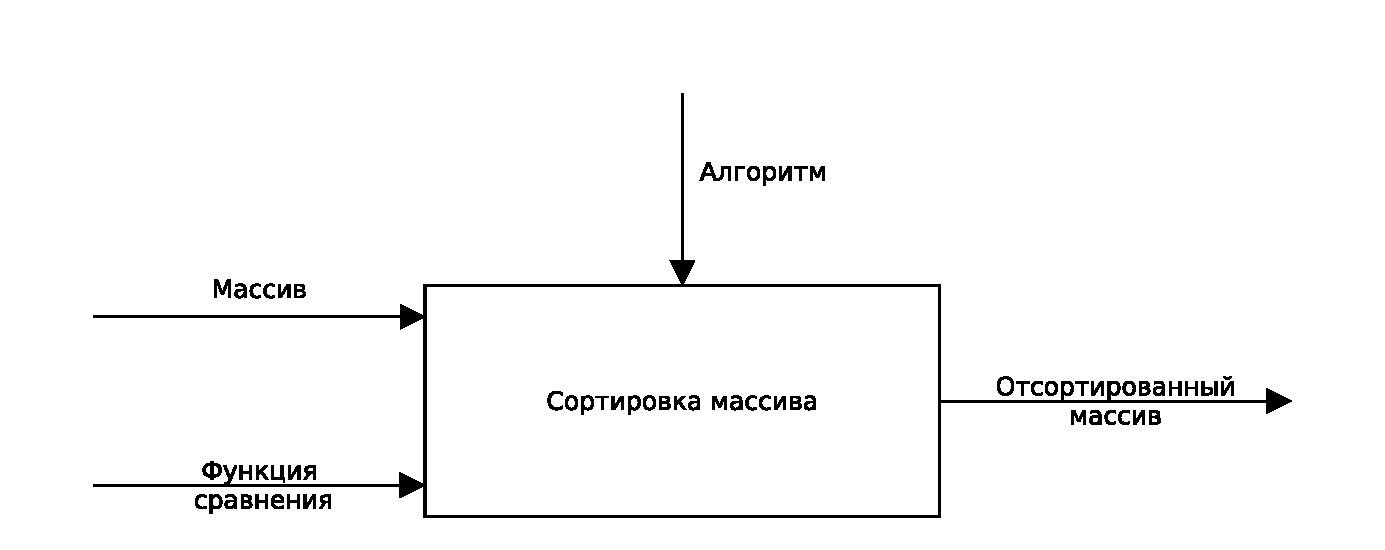
\includegraphics[scale=0.75]{./pdf/mainIdef0.pdf}
    \caption{Функциональная IDEF0 модель уровня 1}
    \label{img:IDEF0}
\end{figure}

\section{Разработка алгоритмов}
Для непосредственной реализации вышеописанных алгоритмов важно иметь их некоторые упрощённые визуальные представления, так как чтение таких представлений упрощает написание кода. Подходящим для этого вариантом визуализации являются схемы алгоритмов.

На рисунках \ref{img:qs}, \ref{img:ins}, \ref{img:shs} изображены схемы алгоритмов быстрой сортировки, сортировки вставками и шейкерной сортировки.

\begin{figure}[H]
    \centering
    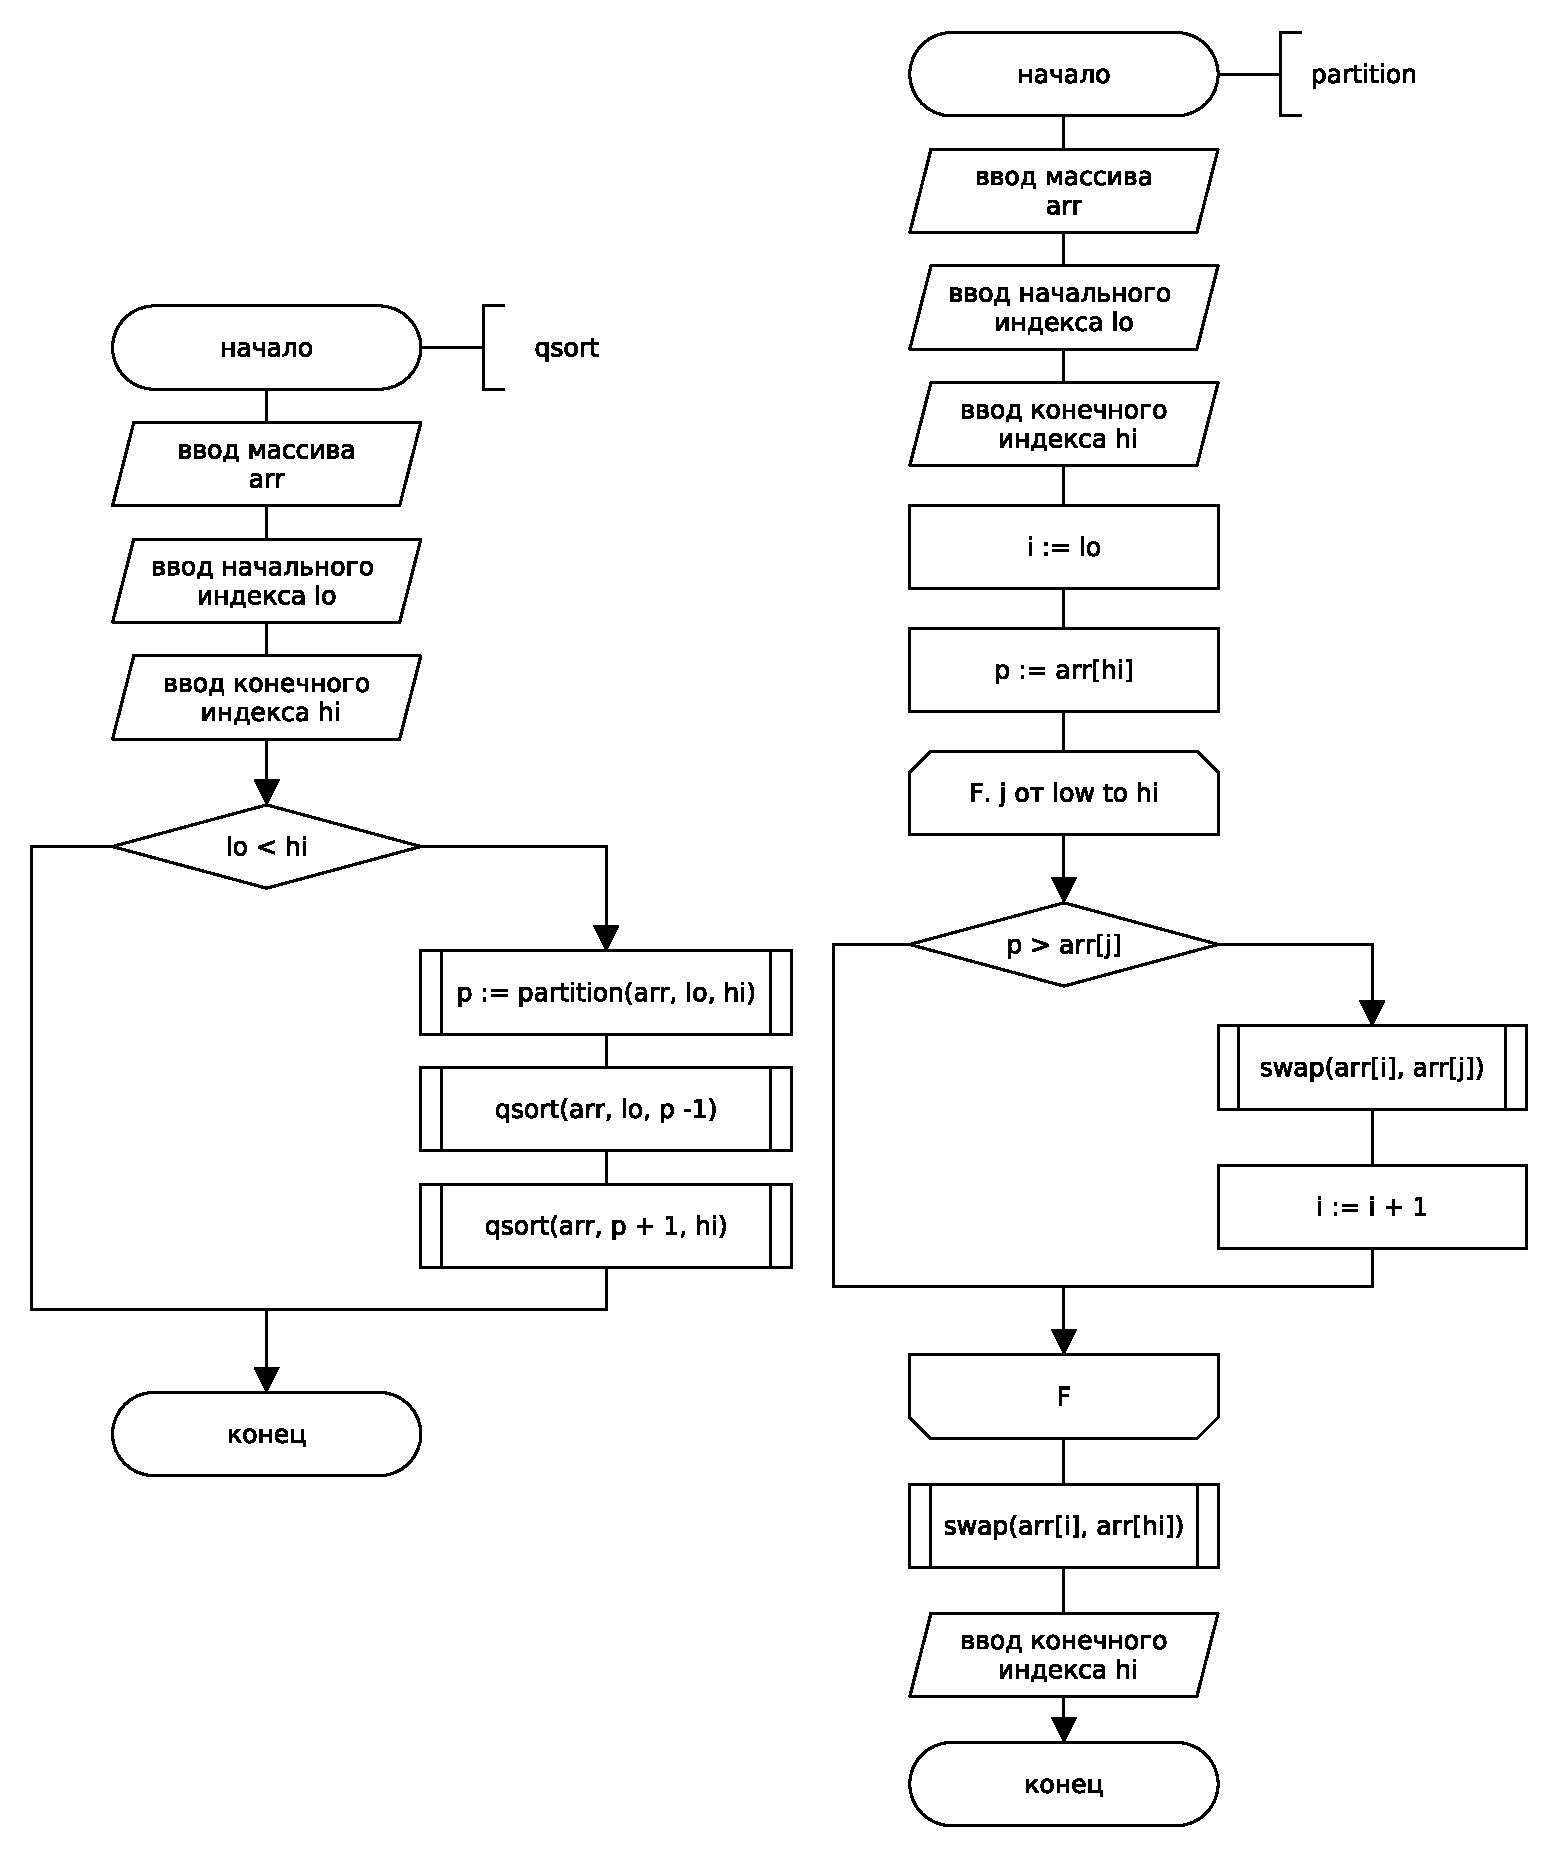
\includegraphics[scale=0.65]{./pdf/qsort.pdf}
    \caption{Быстрая сортровка}
    \label{img:qs}
\end{figure}

\begin{figure}[H]
    \centering
    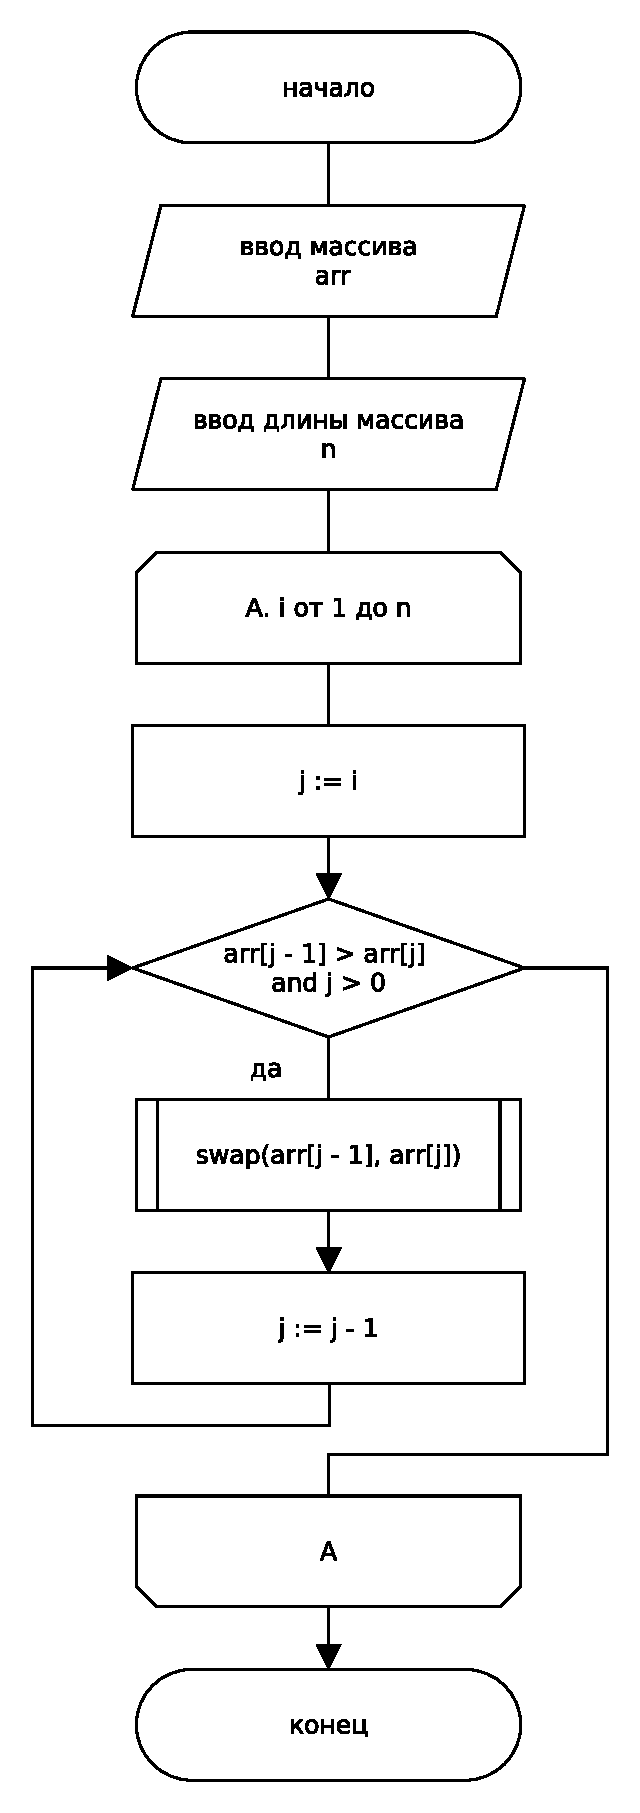
\includegraphics[scale=0.65]{./pdf/insertionsort.pdf}
    \caption{Сортировка вставками}
    \label{img:ins}
\end{figure}

\begin{figure}[H]
    \centering
    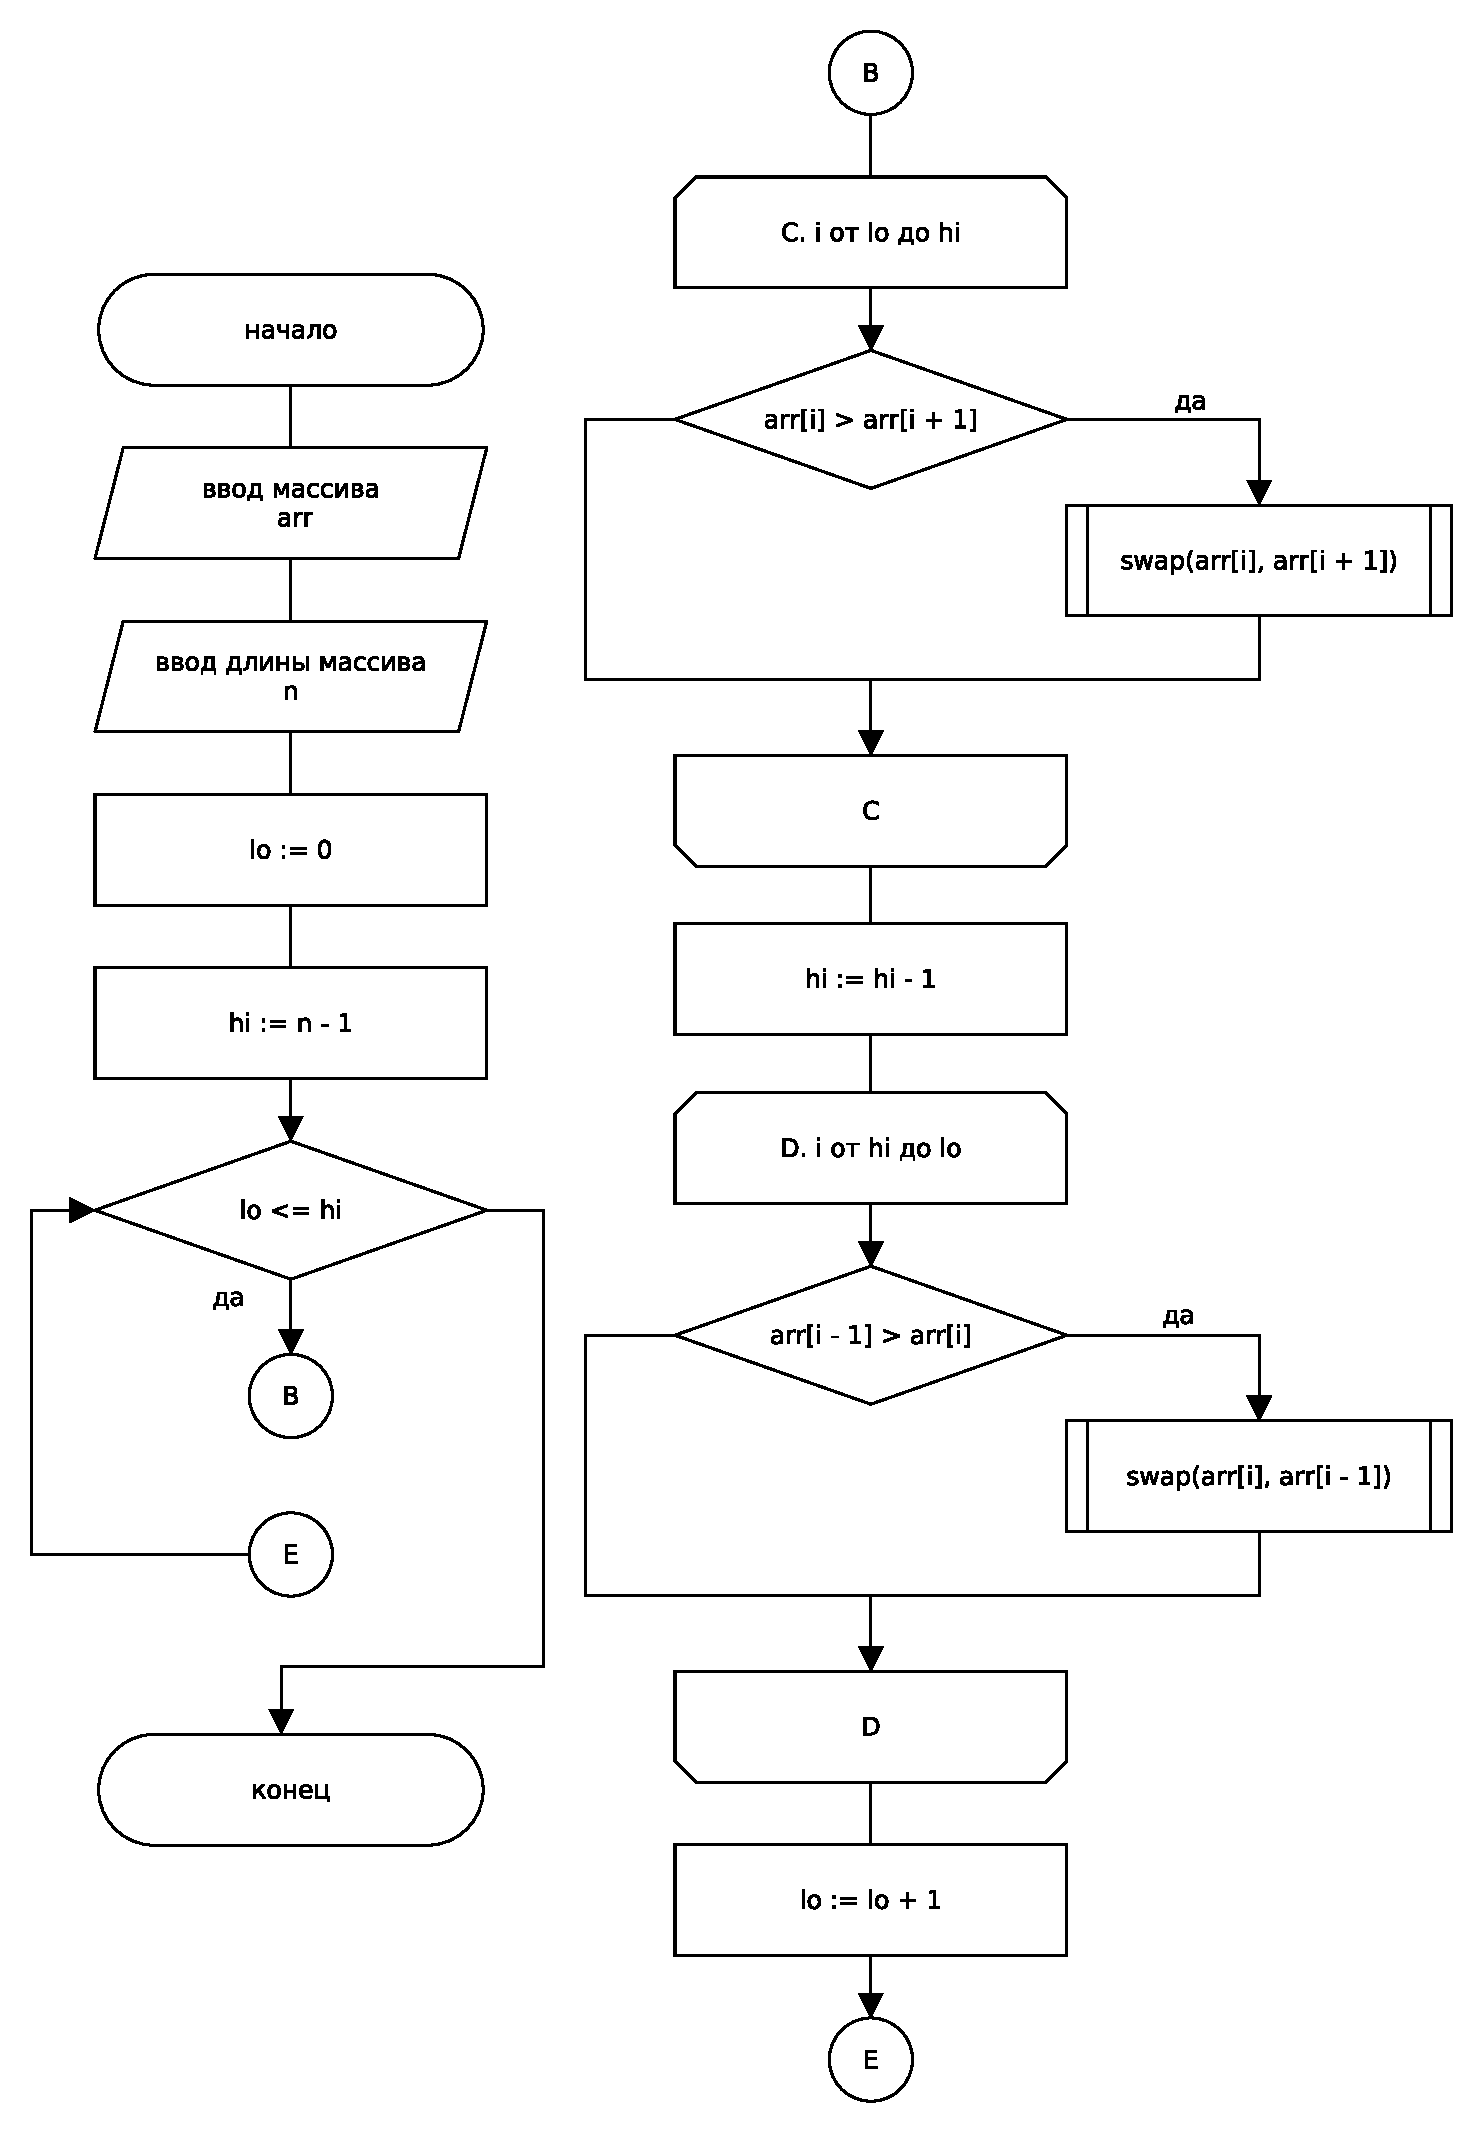
\includegraphics[scale=0.65]{./pdf/shakersort.pdf}
    \caption{Шейкерная сортировка}
    \label{img:shs}
\end{figure}

\section{Трудоемкость алгоритмов}
Проведём оценку сложности рассматриваемых алгоритмов сортировки.

\subsection{Быстрая сортировка}
Для быстрой сортировки с разбиением Ломуто худшими случаями являются случаи с уже отсортированными массивами и обратно отсортированными массивами. В этих условиях сложность составляет $O(n^2)$\cite{knuth}. Так как в контексте задачи сортировки можно рассматривать только три основных вида массивов: отсортированные, отсортированные в обратном порядке, произвольные, а говорить о лучшем случае можно только касательно первых двух видов, так как только для них определено, в каком отношении порядка находятся пары соседних элементов, то лучший случай для быстрой сортировки с разбиением Ломута неопределим. Тогда следует говорить о среднем случае: случае, при котором время выполнения алгоритма является математическим ожиданием. В среднем случае быстрая сортировка с любым разбиением имеет трудоёмкость $O(n\cdot{}log(n))$[1].

\subsection{Сортировка вставками}

\subsection{Шейкерная сортировка}

\section{Вывод}

